\subsection{Results}

\subsubsection{GemNet}

\begin{itemize}
    \item s2ef (batch size 2), is2re(batch size 2)
    \item configurations (8 times): baseline stage 0 (all deepspeed features deactivated), 
    stage 0 fp16: memory savings from deepspeed, not only from fp16. 
    \item big drop from stage 0 to stage 1: Optimizer states have huge influence on
    memory consumption, memory-wise, stage 2 with optimizer offloading best
    \item optimizer offloading saves memory, but increases runtime
    \item stage 3 seems ineffective
    \item communication overlapping (pipeline parallelism) seems ineffective.
\end{itemize}

For each experiment, we performed one epoch of training

\begin{figure}[H]
    \centering

    \begin{subfigure}[t]{0.48\textwidth}
        \centering
        \includegraphics[width=\textwidth]{evaluation/gemnet/s2ef/cuda_memory/memory_comparison.pdf}
        \label{fig:gemnet-s2ef-memory-results}
    \end{subfigure}%
    ~
    \begin{subfigure}[t]{0.48\textwidth}
        \centering
        \includegraphics[width=\textwidth]{evaluation/gemnet/s2ef/runtimes/runtimes_comparison.pdf}
        \label{gemnet-s2ef-runtimes-results}
    \end{subfigure}
    \vspace*{-1.5em}
    \caption{Memory consumption and runtimes on the S2EF task.}
    
\end{figure}

\begin{figure}[H]
    \centering

    \begin{subfigure}[t]{0.48\textwidth}
        \centering
        \includegraphics[width=\textwidth]{evaluation/gemnet/is2re/cuda_memory/memory_comparison.pdf}
        \label{fig:gemnet-is2re-memory-results}
    \end{subfigure}%
    ~
    \begin{subfigure}[t]{0.48\textwidth}
        \centering
        \includegraphics[width=\textwidth]{evaluation/gemnet/is2re/runtimes/runtimes_comparison.pdf}
        \label{gemnet-is2re-runtimes-results}
    \end{subfigure}
    \vspace*{-1.5em}
    \caption{Memory consumption and runtimes on the IS2RE task.}
    
\end{figure}

\subsubsection{DimeNet++}
